\begin{figure*}[!t]
    \centering
    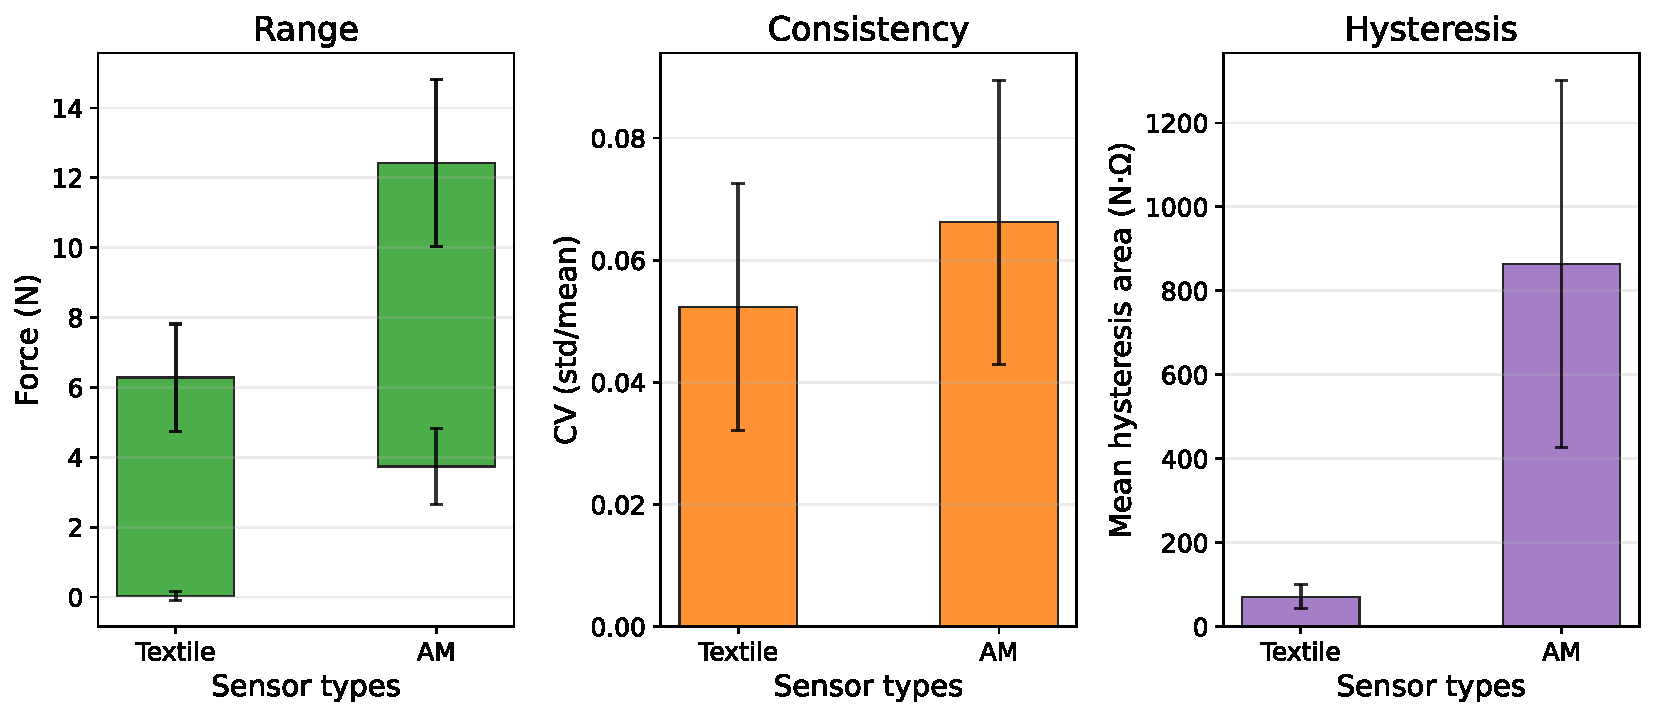
\includegraphics[width=0.85\linewidth]{images/Results/overall_range_repeatability_hysteresis.pdf}
    \caption{ \textbf{Left:} The \textit{Operating Force Range} visualizes the force interval between the minimum detectable force (detection threshold) and the saturation force, which defines the effective range of forces that can be reliably measured by the sensor. \textbf{Middle:} The \textit{Consistency} plot shows the multi-force repeatability metric, which captures the variability of sensor readings across repeated loading cycles at different force levels. \textbf{Right:} The \textit{Hysteresis} plot illustrates the difference between loading and unloading curves, indicating the degree to which the sensor's response depends on its loading history. Together, these plots provide insights into the performance characteristics of the textile and AM sensors. Additional quantitative characterization results are available on the project website.}
    \label{fig:overall_comparison}
\end{figure*}

\section{Sensor Characterization}
\label{sec:characterization}
We characterize both sensor architectures using an Instron testing machine. We use a 1000$\Omega$ reference resistor for the AM sensor and a 47$\Omega$ reference resistor for the textile sensor in a voltage-divider circuit. For each taxel, we apply a 7.5$\times$7.5~mm square applicator at the taxel center and record the voltage response over four load--unload cycles from 0 to 30~N. We fit a power law with base resistance, $R(F)=AF^B+R_{\mathrm{base}}$, to loading and unloading responses and use the fitted curves for performance analysis and force estimation.
To evaluate performance, we report operating force range and consistency metrics.
The project website provides supplementary taxel-level calibration curves, load--unload traces, and quantitative summaries.


\subsection{Operating Force Range} 
We define the operating force range of each sensor as the force interval from its detection threshold (minimum detectable force) to saturation (maximum force for which changes in resistance remain informative). Fig.~\ref{fig:overall_comparison} summarizes the resulting coverage across sensor variants.

\subsubsection{Minimum Detectable Force}
In our pipeline, the detection threshold is measured per taxel as the \emph{break force}:
\[
F_{\mathrm{det}}=\min\{F>0:\; R(F)\le R_{\mathrm{thr}}\},\qquad R_{\mathrm{thr}}=4000~\Omega,
\]

\subsubsection{Saturation Force}
The saturation force is measured from the fitted response $R(F)=AF^B+R_{\mathrm{base}}$ by mapping it through the expected voltage-divider readout
\[
V(F)=V_{\mathrm{in}}\frac{R_{\mathrm{ref}}}{R(F)+R_{\mathrm{ref}}},\qquad V_{\mathrm{in}}=5~\mathrm{V},
\]
and defining
\[
F_{\mathrm{sat}}=\max\Bigl\{F\in[F_{\mathrm{det}},30~\mathrm{N}]:\; \bigl|dV/dF\bigr|\ge 0.03~\mathrm{V/N}\Bigr\},
\]
where $R_{\mathrm{ref}}$ is the reference resistor value, which is selected over a range of reference resistors to find the value that maximizes the sensitive range. We find the optimal value of $R_{\mathrm{ref}}$ is approximately $ R_{\mathrm{base}}$. The sensitive range is $[F_{\mathrm{det}},F_{\mathrm{sat}}]$: below $F_{\mathrm{det}}$ the sensor behaves like an open circuit (negligible signal), while above $F_{\mathrm{sat}}$ the response flattens and force estimates become ambiguous.

\subsubsection{Findings}

Across taxels, the textile sensor operated over approximately 0--6~N, whereas the AM sensor operated over approximately 4--12~N (Fig.~\ref{fig:overall_comparison}, left). Their mean multi-force CVs were approximately 0.052 and 0.066, respectively (Fig.~\ref{fig:overall_comparison}, middle), indicating similar cycle-to-cycle repeatability. The greater AM hysteresis is consistent with deformation of the viscoelastic TPU shell. Together, these results support using the textile configuration for early contact detection and the AM configuration for higher-threshold interactions.

These intervals characterize the tested mechanical configurations and reference resistors rather than intrinsic material limits; changing the mechanical stack or readout resistor will shift the measurable range.

The AM sensor's designed gap explains its elevated detection threshold: as force increases, shell deformation closes the gap and produces a more abrupt resistance transition.

When wrapped on the robot arm and tightened with hook-and-loop fastening, the effective sensitive range of Velostat-based sensors decreases relative to flat characterization. In our tests, mounting primarily reduced the textile sensor's maximum force range. We attribute this reduction to pre-compression and non-uniform pressure distribution across curved surfaces; Velostat bending sensitivity may also shift baseline resistance and response behavior~\cite{11068986}.

Because characterization uses centered normal loads, it does not cover shear, off-center or multi-taxel contact, temperature drift, or long-term cycling; the reported performance is specific to the chosen design parameters and test conditions.


\begin{figure*}[!ht]
    \centering
    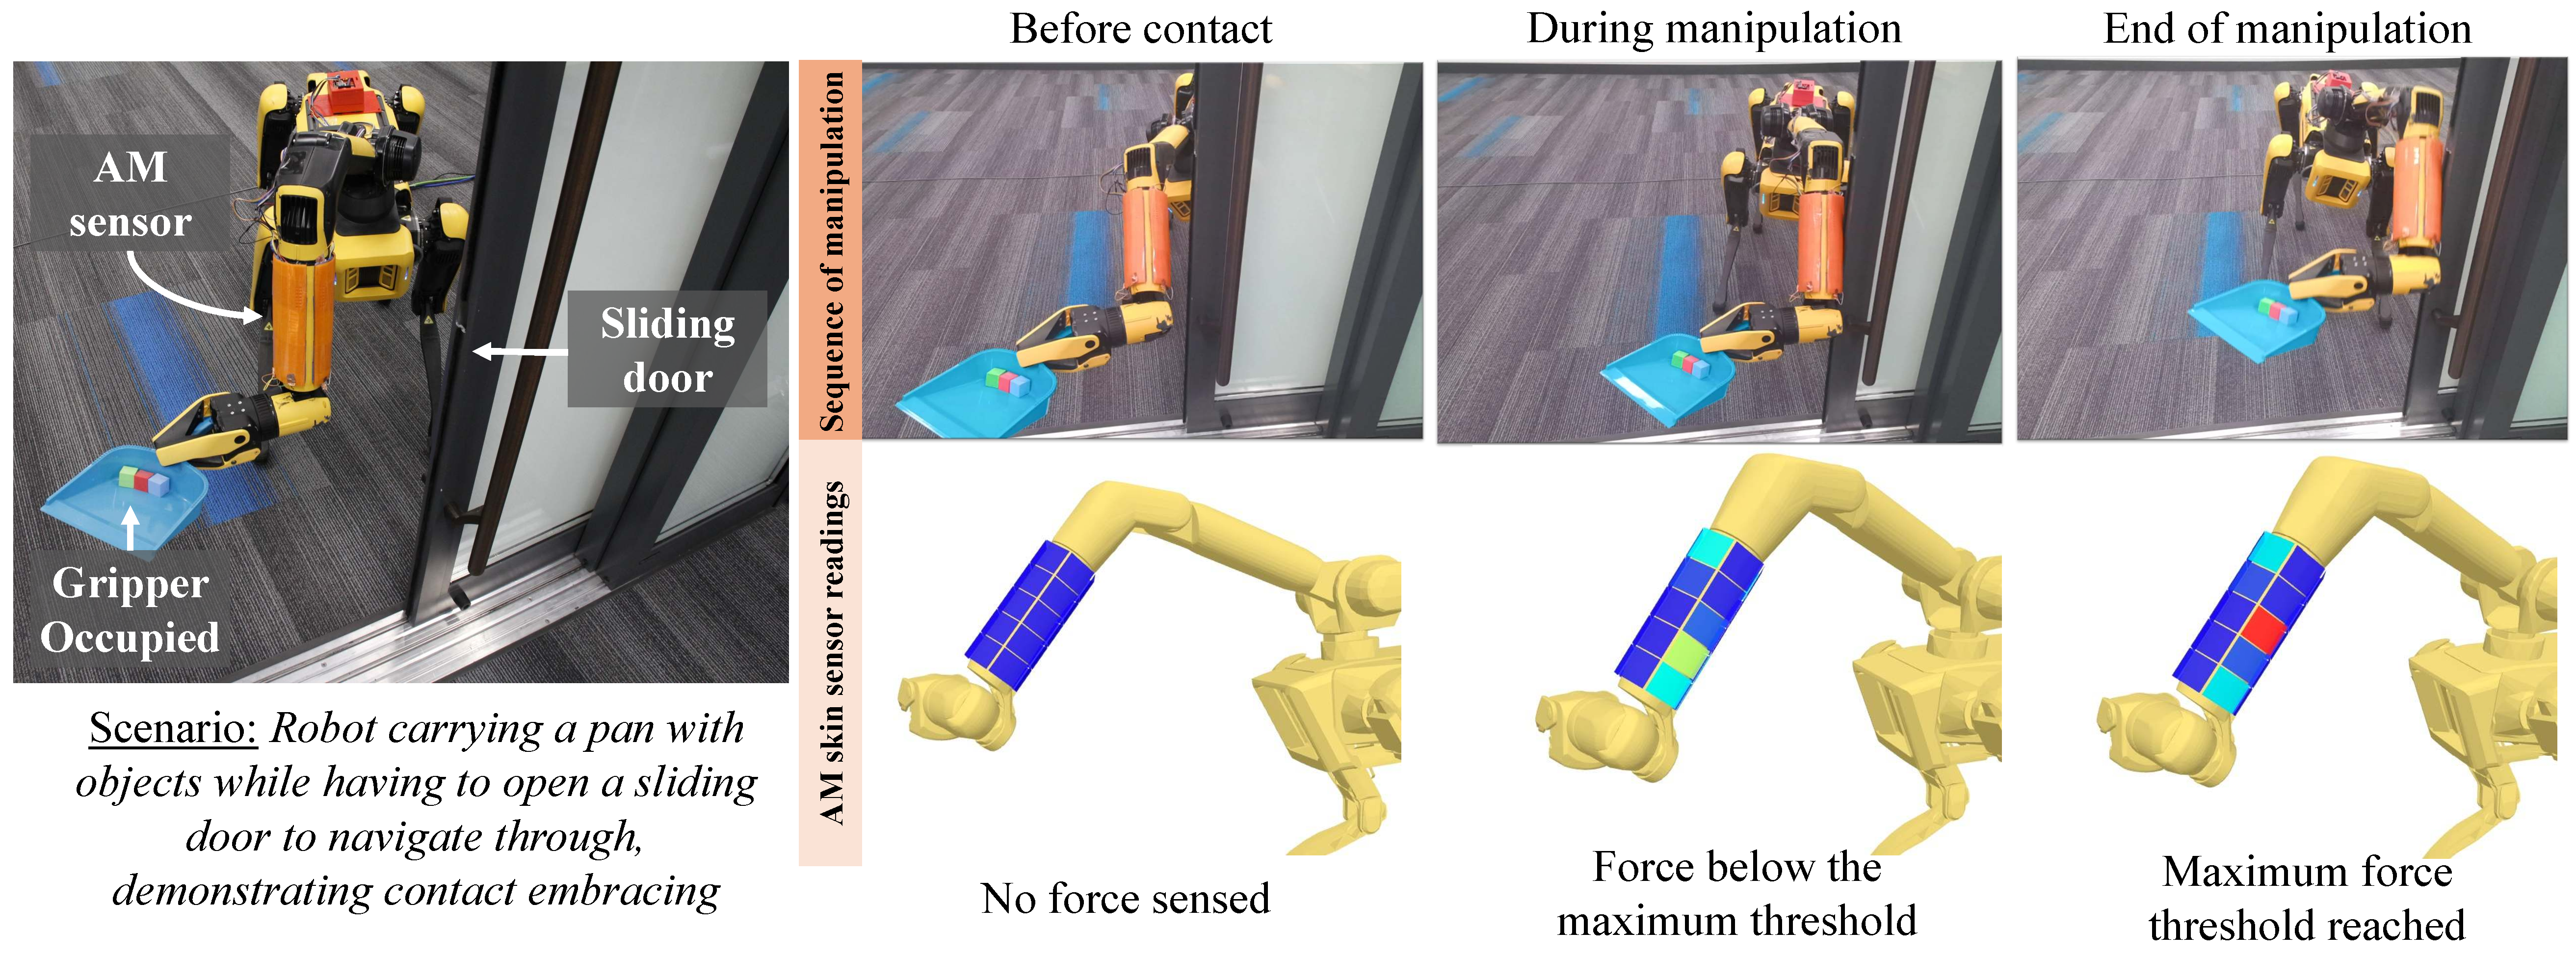
\includegraphics[width=0.95\linewidth]{images/FIg_Embrace_V5.pdf}
    \caption{The contact-embracing task aims to balance a dustpan in the gripper, and open a door while preventing large forces. To open the door, we create a new end effector on the arm of the robot and move along its normal until a force above a threshold is achieved. We also optimize the rotation angle of the gripper to keep the dustpan level.}
    \label{fig:embrace}
 \end{figure*}



\subsection{Consistency}

\subsubsection{Repeatability}
For each taxel, we sample 10 points uniformly across $[F_{\mathrm{det}}, 30~\mathrm{N}]$, and compute the standard deviation of the sensor readings across repeated loading cycles at each force level. We summarize single-force repeatability as the standard deviation $\sigma_R(F)$ of the sensor readings across cycles at each force level $F$:
\begin{equation}
\sigma_R(F) = \mathrm{std}\!\left(\{R_i(F)\}_{i=1}^{N_c}\right),
\end{equation}
along with the corresponding mean $\mu_R(F)$ and the number of valid cycles $N_c$.

To normalize the repeatability metric across different resistances and sensor configurations, we compute the coefficient of variation (CV) across cycles at each force level $F$:

\begin{equation}
\mathrm{CV}(F_j)=\frac{\sigma_R(F_j)}{\mu_R(F_j)}
\end{equation}

We average the CV across each sampled force level to obtain a single multi-force repeatability metric for each taxel:

\begin{equation}
\overline{\mathrm{CV}} = \frac{1}{N_s} \sum_{j=1}^{N_s} \mathrm{CV}(F_j)
\end{equation}

and we then report the mean $\overline{\mathrm{CV}}$ across taxels, along with the corresponding standard deviation across taxels, to summarize the overall repeatability of the sensor. This multi-force repeatability metric captures the consistency of the sensor's response across its operating range and the variability across taxels, providing a comprehensive measure of the sensor's repeatability performance.


% To measure repeatability over each sensor's operating region, we report a multi-force repeatability metric by sampling $N_s=10$ forces (config: \texttt{repeatability\_target\_force\_num\_samples}) uniformly over the overlap of the force ranges observed across cycles, and (optionally) enforcing a minimum-force floor above initial contact: $F \ge F_{\mathrm{det}} + 2~\mathrm{N}$ (config: \texttt{repeatability\_min\_force\_above\_break\_threshold}), where $F_{\mathrm{det}}$ is the break/detection force defined as the minimum force at which $R \le 4000~\Omega$ (config: \texttt{break\_resistance\_threshold\_ohms}). At each sampled force $F_j$, we compute the coefficient of variation
% and summarize multi-force repeatability as the mean $\overline{\mathrm{CV}}$ across the sampled forces.

\subsubsection{Hysteresis}
We quantify hysteresis using the discrepancy between the loading and unloading curves in the resistance domain. For each taxel, we fit power-law models to the loading and unloading data,
\begin{equation}
R(F)=AF^B+R_{\mathrm{base}},
\end{equation}
and invert them to obtain $F_{\text{load}}(R)$ and $F_{\text{unload}}(R)$ over the region where inversion is valid. Hysteresis is then computed as the area between the two inverted curves:
\begin{equation}
H_{\text{area}} = \int_{R_{\text{min}}}^{R_{\text{max}}} \left|F_{\text{load}}(R) - F_{\text{unload}}(R)\right| \, dR,
\end{equation}
 This area-based metric captures cumulative hysteretic behavior across the operating range, rather than at a single point.


\subsubsection{Findings}
The greater AM hysteresis (Fig.~\ref{fig:overall_comparison}, right) is attributed primarily to viscoelastic effects in the printed shell; the textile sensor shows less separation between loading and unloading curves under these test conditions.
